\chapter{Manutenzione}
\label{Manutenzione}
\thispagestyle{empty}

In questa capitolo si spiega come provvedere a conservare lo stato dell'installazione locale di ShareLaTeX. È necessario pianificare le attività di ripristino dei dati del sistema in quanto l'avvio dei container con immagini aggiornate potrebbe impedire il corretto funzionamento del sistema o la perdita di dati e documenti finora creati. Si ricorda inoltre che un semplice riavvio dei container comporta il loro ripristino.

\section{Backup e ripristino}
Il \hyperref[code:docker-compose.yml]{template} di \verb|docker-compose.yml| mostrato nel capitolo \hyperref[Installazione]{\enquote*{Installazione}} possiede già impostazioni riguardanti la persistenza dei dati dei tre container installati. Saranno aggiunte altre impostazioni per rendere più sicura la procedura di aggiornamento del sistema in futuro.

\subsection{ShareLaTeX}
I dati relativi a ShareLaTeX sono salvati all'interno del container in \verb|/var/lib/sharelatex| e il template di \verb|docker-compose.yml| crea di default un volume per la persistenza dei dati.
\begin{lstlisting}
volumes:
    - ~/sharelatex_data:/var/lib/sharelatex
\end{lstlisting}

\subsection{MongoDB}
MongoDB possiede due tool chiamati \verb|mongodump| e \verb|mongorestore| che saranno utilizzati per esportare ed importare il dataset in un formato sicuro per il backup. Per ulteriori informazioni visitare la documentazione ufficiale di MongoDB all'indirizzo \url{docs.mongodb.com/manual/tutorial/backup-and-restore-tools/}. Innanzitutto eseguire \verb|mongodump|.
\begin{lstlisting}
sudo docker exec mongo mongodump
\end{lstlisting}
L'output sarà all'interno del container MongoDB in \verb|/dump|. Per rendere questi file persistenti occorre montare un volume esterno. Si noti che Il template di \verb|docker-compose.yml| crea di default un volume per la persistenza dei dati, che non è sufficiente in caso di upgrade o downgrade di MongoDB.
\begin{lstlisting}
volumes:
    - ~/mongo_data:/data/db
    - ~/mongodump_data:/dump
\end{lstlisting}
Riavviando il container, l'output di \verb|mongodump| sarà accessibile nella home directory dell'host. Con \verb|mongorestore| sarà poi possibile ripristinare lo stato di MongoDB.
\begin{lstlisting}
sudo docker exec mongo mongorestore /dump
\end{lstlisting}

\subsection{Redis}
Redis è utilizzato come meccanismo di caching, per cui contiene dati a breve termine, ma può essere comunque importante eseguire un backup dei dati. Il template di \verb|docker-compose.yml| crea di default un volume per la persistenza dei dati. Conterrà un unico file nominato \verb|dump.rdb|.
\begin{lstlisting}
volumes:
    - ~/redis_data:/data
\end{lstlisting} 

\subsection{Ridondanza della memoria del sistema}
Il server su cui è stata installata la macchina \verb|sharelatex| possiede storage con RAID. Guasti sulla macchina virtuale non comprometteranno lo stato del servizio, dei profili utente e dei progetti, in quanto la ridondanza introdotta permette il ripristino della macchina in caso di failure.

\section{Aggiornamento}
Una volta eseguiti i passi per gestire l'operazione di backup e ripristino, è necessario definire gli step per eseguire l'upgrade (o downgrade) dei container in modo sicuro, senza perdita di dati.

\subsection{Logout degli utenti}
È opportuno impedire agli utenti di utilizzare l'applicazione durante la fase di aggiornamento. Per far ciò l'amministratore deve fare login e accedere al pannello di gestione del sito presso \verb|sharelatex.ing.unimore.it/admin|.
\begin{figure}[h]
    \centering
    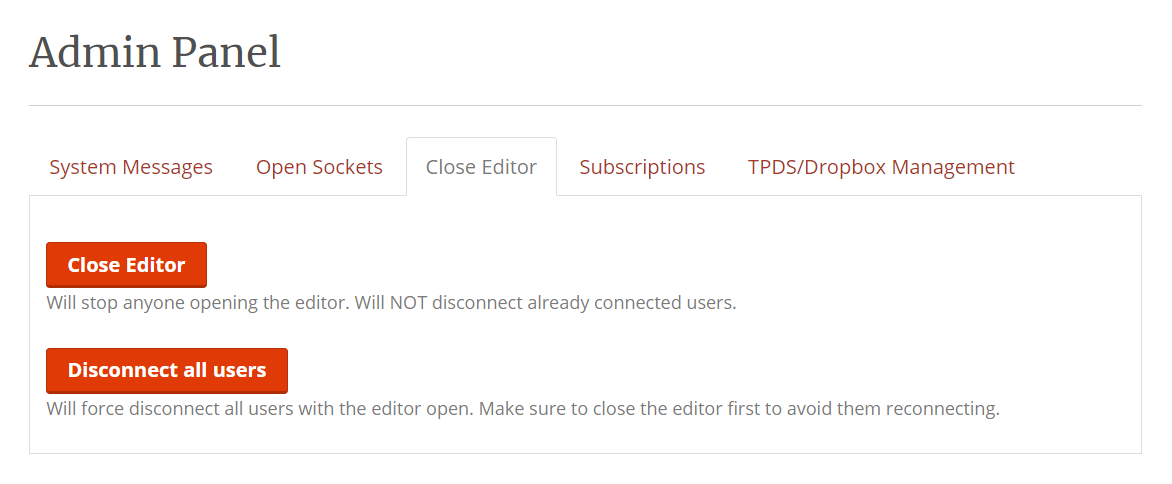
\includegraphics[width=\textwidth]{immagini/close_editor.PNG}
    \caption{Pannello di controllo dell'amministratore}
    \label{fig:close_editor}
\end{figure}
\begin{enumerate}
    \item Accedere alla scheda \enquote*{Close Editor}.
    \item Cliccare sul bottone \enquote*{Close Editor}: impedisce agli utenti di caricare l'editor di progetto.
    \item Cliccare sul bottone \enquote*{Disconnect all users}: chiunque sia connesso all'editor verrà rinviato ad una pagina di avviso manutenzione.
\end{enumerate}
L'unico modo per riavviare l'editor consiste nel riavvio dei container.

\subsection{Esecuzione di mongodump}
Per eseguire il backup dei dati di MongoDB bisogna eseguire \verb|mongodump|. Non sarà necessario conservare la directory \verb|mongo_data| in quanto \verb|mongorestore| sarà in grado di ripristinarla a dovere. L'output di \verb|mongodump| avverrà in \verb|/dump| all'interno del container. Avendo montato un volume in \verb|~/mongodump_data|, tale percorso sarà accessibile dall'esterno del container e persistente.
\begin{lstlisting}
sudo docker exec mongo mongodump
\end{lstlisting}

\subsection{Sospensione e rimozione dei container}
Si può scegliere se agire su tutti e tre i container o solo sul container da aggiornare.
\begin{lstlisting}
sudo docker stop sharelatex mongo redis
sudo docker rm sharelatex mongo redis
\end{lstlisting}

\subsection{Rimozione dei dati precedenti}
Eliminare la directory sull'host \verb|mongo_data|. È necessario in quanto i container possono rifiutare l'avvio con dati diversi: è il caso di MongoDB. Non bisogna eliminare invece la directory sull'host \verb|mongodump_data| perché frutto del montaggio di un volume esterno necessario per eseguire \verb|mongorestore|.
\begin{lstlisting}
sudo rm -r ~/mongo_data
\end{lstlisting}
Se al successivo riavvio del sistema il container Redis dovesse rifiutare il riavvio, aggiungere agli step precedenti l'eliminazione della diretory sull'host \verb|redis_data|.
\begin{lstlisting}
sudo rm -r ~/redis_data
\end{lstlisting}

\subsection{Riavvio del sistema}
Il template di \verb|docker-compose.yml| imposta come immagine di default per ogni container quella con tag \verb|latest|. È possibile anche selezionare una specifica immagine da scaricare. L'elenco delle immagini disponibili è su Docker Hub. Ad esempio, se si vuole l'immagine \verb|v1.0.0| di ShareLaTeX è necessario appendere il tag selezionato nel campo \verb|image| mediante \verb|:|. Segue un esempio di quanto detto.
\begin{lstlisting}
services:
    sharelatex:
        restart: always
        image: sharelatex/sharelatex:v1.0.0
        container_name: sharelatex
\end{lstlisting}
Quindi riavviare i container.
\begin{lstlisting}
sudo docker-compose up -d
\end{lstlisting}

\subsection{Ripristino con mongorestore}
Si presenterà una nuova installazione dell'applicazione. Per ripristinare i dati precedenti occorre eseguire \verb|mongorestore|.
\begin{lstlisting}
sudo docker exec mongo mongorestore /dump
\end{lstlisting}

\section{Agevolazione degli aggiornamenti: update.sh}
Per agevolare il processo di aggiornamento dei container è stato prodotto lo script \verb|update.sh|. Questo script esegue il procedimento precedentemente descritto passo per passo, mostrando all'utente lo stato di ogni fase. Per eseguire lo script è necessario scaricarlo e ottenere i permessi di esecuzione.
\begin{lstlisting}
wget https://raw.githubusercontent.com/aimagelab/sharelatex/master/update.sh
chmod +x update.sh
\end{lstlisting}
Lo script accetta un parametro che identifica una directory. Tale directory deve contenere un file \verb|docker-compose.yml| da utilizzare per avviare e configurare i container.
\begin{lstlisting}
./update.sh <dir>
\end{lstlisting}
Avendo inserito tale file in una directory chiamata \verb|sharelatex|, il comando sarà il seguente.
\begin{lstlisting}
./update.sh sharelatex
\end{lstlisting}
Lo script controlla innanzitutto il numero dei parametri: se non sufficiente, allora lo notifica all'utente. Esegue quindi un controllo sul parametro, per verificare che identifichi una directory traversabile. Segue eseguendo \verb|mongodump|, arrestando i container, eliminando i dati superflui, riavviando i container, per poi ripristinare i dati con \verb|mongorestore|. Mostra infine lo stato attuale dei container attivi e chiede all'utente se proseguire con l'installazione completa (o aggiornamento) di TeX Live.

Si raccomanda di utilizzare questo script anche in caso di semplice riavvio dei container: dato che è stato impostato in \verb|docker-compose.yml| che l'immagine da utilizzare per la creazione dei container è quella con tag \enquote*{latest}, l'eventuale release di un'immagine aggiornata comporterebbe il suo download e la sostituzione con l'immagine precedente, il che costituisce un vero e proprio aggiornamento.

Segue lo script \verb|update.sh|.
\lstinputlisting[caption={Script update.sh}, captionpos=b, style=my-style]{script/update-ridotto.sh}